\documentclass[preprint, 3p,
authoryear]{elsarticle} %review=doublespace preprint=single 5p=2 column
%%% Begin My package additions %%%%%%%%%%%%%%%%%%%

\usepackage[hyphens]{url}

  \journal{Momento: Diálogos em Educação} % Sets Journal name

\usepackage{graphicx}
%%%%%%%%%%%%%%%% end my additions to header

\usepackage[T1]{fontenc}
\usepackage{lmodern}
\usepackage{amssymb,amsmath}
% TODO: Currently lineno needs to be loaded after amsmath because of conflict
% https://github.com/latex-lineno/lineno/issues/5
\usepackage{lineno} % add
\usepackage{ifxetex,ifluatex}
\usepackage{fixltx2e} % provides \textsubscript
% use upquote if available, for straight quotes in verbatim environments
\IfFileExists{upquote.sty}{\usepackage{upquote}}{}
\ifnum 0\ifxetex 1\fi\ifluatex 1\fi=0 % if pdftex
  \usepackage[utf8]{inputenc}
\else % if luatex or xelatex
  \usepackage{fontspec}
  \ifxetex
    \usepackage{xltxtra,xunicode}
  \fi
  \defaultfontfeatures{Mapping=tex-text,Scale=MatchLowercase}
  \newcommand{\euro}{€}
\fi
% use microtype if available
\IfFileExists{microtype.sty}{\usepackage{microtype}}{}
\usepackage[]{natbib}
\bibliographystyle{elsarticle-harv}

\ifxetex
  \usepackage[setpagesize=false, % page size defined by xetex
              unicode=false, % unicode breaks when used with xetex
              xetex]{hyperref}
\else
  \usepackage[unicode=true]{hyperref}
\fi
\hypersetup{breaklinks=true,
            bookmarks=true,
            pdfauthor={},
            pdftitle={Short Paper},
            colorlinks=false,
            urlcolor=blue,
            linkcolor=magenta,
            pdfborder={0 0 0}}

\setcounter{secnumdepth}{5}
% Pandoc toggle for numbering sections (defaults to be off)

% Pandoc syntax highlighting
\usepackage{color}
\usepackage{fancyvrb}
\newcommand{\VerbBar}{|}
\newcommand{\VERB}{\Verb[commandchars=\\\{\}]}
\DefineVerbatimEnvironment{Highlighting}{Verbatim}{commandchars=\\\{\}}
% Add ',fontsize=\small' for more characters per line
\usepackage{framed}
\definecolor{shadecolor}{RGB}{248,248,248}
\newenvironment{Shaded}{\begin{snugshade}}{\end{snugshade}}
\newcommand{\AlertTok}[1]{\textcolor[rgb]{0.94,0.16,0.16}{#1}}
\newcommand{\AnnotationTok}[1]{\textcolor[rgb]{0.56,0.35,0.01}{\textbf{\textit{#1}}}}
\newcommand{\AttributeTok}[1]{\textcolor[rgb]{0.13,0.29,0.53}{#1}}
\newcommand{\BaseNTok}[1]{\textcolor[rgb]{0.00,0.00,0.81}{#1}}
\newcommand{\BuiltInTok}[1]{#1}
\newcommand{\CharTok}[1]{\textcolor[rgb]{0.31,0.60,0.02}{#1}}
\newcommand{\CommentTok}[1]{\textcolor[rgb]{0.56,0.35,0.01}{\textit{#1}}}
\newcommand{\CommentVarTok}[1]{\textcolor[rgb]{0.56,0.35,0.01}{\textbf{\textit{#1}}}}
\newcommand{\ConstantTok}[1]{\textcolor[rgb]{0.56,0.35,0.01}{#1}}
\newcommand{\ControlFlowTok}[1]{\textcolor[rgb]{0.13,0.29,0.53}{\textbf{#1}}}
\newcommand{\DataTypeTok}[1]{\textcolor[rgb]{0.13,0.29,0.53}{#1}}
\newcommand{\DecValTok}[1]{\textcolor[rgb]{0.00,0.00,0.81}{#1}}
\newcommand{\DocumentationTok}[1]{\textcolor[rgb]{0.56,0.35,0.01}{\textbf{\textit{#1}}}}
\newcommand{\ErrorTok}[1]{\textcolor[rgb]{0.64,0.00,0.00}{\textbf{#1}}}
\newcommand{\ExtensionTok}[1]{#1}
\newcommand{\FloatTok}[1]{\textcolor[rgb]{0.00,0.00,0.81}{#1}}
\newcommand{\FunctionTok}[1]{\textcolor[rgb]{0.13,0.29,0.53}{\textbf{#1}}}
\newcommand{\ImportTok}[1]{#1}
\newcommand{\InformationTok}[1]{\textcolor[rgb]{0.56,0.35,0.01}{\textbf{\textit{#1}}}}
\newcommand{\KeywordTok}[1]{\textcolor[rgb]{0.13,0.29,0.53}{\textbf{#1}}}
\newcommand{\NormalTok}[1]{#1}
\newcommand{\OperatorTok}[1]{\textcolor[rgb]{0.81,0.36,0.00}{\textbf{#1}}}
\newcommand{\OtherTok}[1]{\textcolor[rgb]{0.56,0.35,0.01}{#1}}
\newcommand{\PreprocessorTok}[1]{\textcolor[rgb]{0.56,0.35,0.01}{\textit{#1}}}
\newcommand{\RegionMarkerTok}[1]{#1}
\newcommand{\SpecialCharTok}[1]{\textcolor[rgb]{0.81,0.36,0.00}{\textbf{#1}}}
\newcommand{\SpecialStringTok}[1]{\textcolor[rgb]{0.31,0.60,0.02}{#1}}
\newcommand{\StringTok}[1]{\textcolor[rgb]{0.31,0.60,0.02}{#1}}
\newcommand{\VariableTok}[1]{\textcolor[rgb]{0.00,0.00,0.00}{#1}}
\newcommand{\VerbatimStringTok}[1]{\textcolor[rgb]{0.31,0.60,0.02}{#1}}
\newcommand{\WarningTok}[1]{\textcolor[rgb]{0.56,0.35,0.01}{\textbf{\textit{#1}}}}

% tightlist command for lists without linebreak
\providecommand{\tightlist}{%
  \setlength{\itemsep}{0pt}\setlength{\parskip}{0pt}}

% From pandoc table feature
\usepackage{longtable,booktabs,array}
\usepackage{calc} % for calculating minipage widths
% Correct order of tables after \paragraph or \subparagraph
\usepackage{etoolbox}
\makeatletter
\patchcmd\longtable{\par}{\if@noskipsec\mbox{}\fi\par}{}{}
\makeatother
% Allow footnotes in longtable head/foot
\IfFileExists{footnotehyper.sty}{\usepackage{footnotehyper}}{\usepackage{footnote}}
\makesavenoteenv{longtable}






\begin{document}


\begin{frontmatter}

  \title{Short Paper}
    \author[Universidade Federal do Rio Grande]{Sheron Magalhães dis
Santos%
  \corref{cor1}%
  \fnref{1}}
   \ead{sher.off21@gmail.com} 
      \affiliation[Instituto de Matemática, Estatística e Física -
IMEF]{
    organization={Universidade Federal do Rio Grande -
FURG},addressline={Av Itália, km 8, s/n},city={Rio
Grande},postcode={96213220},state={Rio Grande do Sul},country={Brasil},}
    \affiliation[Another University]{
    }
    \cortext[cor1]{Corresponding author}
    \fntext[1]{This is the first author footnote.}
    \fntext[2]{Another author footnote.}
  
  \begin{abstract}
  This article results from a research carried out in the Scientific
  Electronic Library Online -- SciELO and in the Nota Qualis-Periódicos
  section of the Plataforma Sucupira, specifically in the data for the
  2017-2020 quadrennium. Applying the expressions ``Assistive
  Technology'' and ``inclusion education technology'', the results were
  filtered so that only national and Portuguese-language publications
  were displayed, referring to years 2018 to 2022. Was built a
  theoretical map with the search results, which totaled sixteen
  articles, intending to understand the state of knowledge about
  inclusive technologies for People with Disabilities (PwD) within the
  school environment. In the process of recognition and analysis, these
  articles were separated into three categories according to suggestions
  for implementation, maintenance, and quality of inclusion of
  Technologies in that context. It was possible to verify with the
  research that the nature and magnitude of the effect of the practice
  of inclusive education through the use of technologies depend on some
  factors such as teacher training, the inclusion of Assistive
  Technology (AT), and special education professionals in the school
  environment. It is also of notorious importance that the literature on
  the subject in question continues to be researched and produced, to
  build knowledge so that educational technologies with inclusive
  content are elaborated and implemented.It was also noticeable that the
  production of the use of at to promote the inclusion of PwD students
  is still limited, and it is important to encourage study and research
  within schools, universities, and other social spaces that are
  interested in the subject.
  \end{abstract}
    \begin{keyword}
    Assistive
Technology \sep Inclusion \sep Acessibility \sep Education \sep 
    Theoretical map
  \end{keyword}
  
 \end{frontmatter}

\section{Introdução}\label{introduuxe7uxe3o}

A inclusão de Pessoas com Deficiência (PcDs) é um interesse crescente
desde muito tempo e, no Brasil, se materializa a partir da a criação da
Lei Brasileira de Inclusão da Pessoa com Deficiência ou Estatuto da
Pessoa com Deficiência, sob o nº 13.146 de 06 de julho de 2015. A partir
dessa Lei, os indivíduos que antes eram tratados como portadores de
necessidades especiais ou excepcionais passaram a se constituir como
sujeitos de direito, dentre eles, o direito à educação. Para Miranda e
Galvão (2012), além da necessidade de cumprir a legislação em vigor, é
importante criar oportunidades de ensino e aprendizagem aos discentes
com deficiência, a fim de tornar tangível a sua participação no processo
educativo e científico, evitando que haja barreiras que impeçam o
desenvolvimento do conhecimento e da sua formação.

Garantir o acesso à educação inclusiva e de qualidade, bem como
possibilitar chances de aprendizagem ao decorrer da vida para todos até
2030 é uma das finalidades fundamentais da Organização das Nações Unidas
(ONU), que é citado na agenda de desenvolvimento sustentável pós 2015.
Na Resolução nº 02 de 1º de julho de 2015, do Conselho Nacional de
Educação (CNE), o qual define as ``Diretrizes Curriculares Nacionais
para a formação inicial em nível superior (cursos de licenciatura,
cursos de formação pedagógica para graduados e cursos de segunda
licenciatura) e para a formação continuada'', faz-se, também, referência
à inclusão (BRASIL, 2015).

Além disso, é importante evidenciar que há, no momento, transformações
sociais aceleradas em diferentes áreas. Nesse contexto surge a
Tecnologia Assistiva (TA), que é uma área do conhecimento e de atuação
na qual são desenvolvidos serviços, recursos e estratégias que têm como
objetivo contribuir na resolução ou minimizar dificuldades funcionais de
PcDs na realização de tarefas (SARTORETTO; BERSCH, 2010). Assim, é
importante citar que tecnologias não são necessariamente instrumentos
digitais, assim, considera-se como TA toda e qualquer inovação que tenha
como utilidade e objetivo a inclusão e acessibilidade de pessoas com
deficiência.

Segundo Kenski, a internet trouxe mudanças irreversíveis para a
sociedade nas últimas décadas, fazendo com que instituições de todos os
setores alterem suas práticas, ações e comunicações (KENSKI, 2015).
Dessa forma, segundo Galvão (2009), ganham força correntes humanistas
que defendem a valorização das diferenças, indicando a importância da
verdadeira inclusão social de todos. Assim, tendo em vista os avanços
percebidos na sociedade, é crescente a criação de pesquisas relacionadas
à Tecnologia Assistiva, que, ainda na mesma obra, o autor defende como
uma ferramenta fundamental para a autonomia e inclusão escolar e social
de PcDs.

Frente ao movimento de pesquisas para consolidação e manutenção da
inclusão escolar de PcDs através do uso de tecnologias, a realização de
pesquisas pode contribuir para o avanço do conhecimento científico na
área. Logo, no contexto do Programa de Pós-graduação em Ciências
Computacionais -- PPGCOMP da Universidade Federal do Rio Grande - FURG,
a presente escrita é estruturada a partir de uma provocação e do
movimento de pesquisa proposto pela disciplina de Fundamentos em
Tecnologias Educacionais.

Na referida proposta, os discentes foram incentivados a realizar o
estado do conhecimento sobre alguma temática de interesse, que tivesse
relação com o ensino e as tecnologias. Ao encontro dessa orientação,
optou-se pela temática ``uso de tecnologias educacionais inclusivas para
pessoas com deficiência'' e o espaço de busca escolhido foi a biblioteca
virtual Scientific Electronic Library Online - SciELO. Uma vez definidos
a temática e o espaço de busca, foi escolhida como metodologia o mapa
teórico, que para Biembengut (2008), é ferramenta essencial para a
estruturação da justificativa de uma pesquisa científica. A construção
de um mapa teórico consiste na revisão de literatura disponível dos
conceitos e das definições sobre o tema de interesse, e é dividida em
três etapas processuais -- identificação, classificação/organização e
reconhecimento/análise (BIEMBENGUT, 2008). Os passos anteriormente
citados podem ser resumidos no ato de identificar as publicações
existentes por meio de palavras-chave, organizar e classificar as mesmas
de acordo com critérios escolhidos pelo pesquisador e analisar os
conceitos teóricos e resultados principais. Dessa forma, considera-se
que o mapa teórico é capaz de identificar as pesquisas acadêmicas
recentes desenvolvidas no campo de análise. Assim, seguindo os
procedimentos dessa metodologia, é possível justificar a relevância de
uma investigação, a partir dos artigos selecionados ou descartados nas
diferentes etapas.

Nessa perspectiva, a elaboração da pesquisa parte da premissa de que
entender o estado do conhecimento sobre as tecnologias educacionais
inclusivas de pessoas com deficiência é significativo no processo de
formação do professor e do pesquisador. Assim, assume-se como objetivo
desse artigo a construção de um mapa teórico acerca do estado do
conhecimento sobre o uso de tecnologias educacionais para a inclusão de
PcDs nas escolas. Segundo a já referenciada autora, ``{[}\ldots{]} ao
mapear estas pesquisas acadêmicas vamos dispondo de vasto domínio sobre
o conhecimento existente na área em questão.'' (BIEMBENGUT, 2008, p.98).

\section{Caminhos metodológicos}\label{caminhos-metodoluxf3gicos}

Dentro da proposta de realizar uma revisão sistemática acerca da
utilização de tecnologias para inclusão de pessoas com deficiência nas
escolas, foi organizado um mapa teórico para classificação dos artigos.
Neste processo de identificação das escritas, realizou-se uma busca na
biblioteca eletrônica SciELO, com os termos ``Tecnologia Assistiva'' e
``tecnologia educação inclusão''. Na busca, foram aplicados os filtros
de pesquisa para artigos nacionais e em língua portuguesa, publicados
entre os anos de 2018 e 2022. Nessa etapa investigativa, identificou-se
cinquenta e três artigos, e ainda no mesmo escopo, foram selecionadas
publicações que tinham como objetivo mapear relatos e reflexões sobre
inclusão e acessibilidade para PcDs, visto que muitas publicações
encontradas citavam outros tipos de inclusão. No final deste processo
foi contabilizado um total de trinta e cinco artigos.

Identificados os artigos que versavam sobre inclusão e acessibilidade de
PcDs, seus resumos foram lidos com o objetivo de selecionar aqueles que
tinham ênfase na educação inclusiva. O processo de leitura dos resumos
colocou em evidência dezoito publicações. Em seguida foi realizada uma
nova pesquisa, desta vez na Plataforma Sucupira, mais especificamente na
avaliação dos periódicos do quadriênio 2017 -- 2020. Nessa etapa, o
objetivo era conhecer os Qualis das revistas/periódicos, com o interesse
de considerar apenas A1, A2, A3 e A4. Na pesquisa, constatou-se que
treze dos dezoito artigos atendiam esse requisito, sendo dez deles
publicados em revistas/periódicos com Qualis A1, três com Qualis A2, e
nenhum deles publicado em revistas ou periódicos avaliados como A3 ou A4
na plataforma.

A etapa de classificação e organização iniciou com a criação de um único
arquivo, o qual continha os resumos e as palavras-chave dos treze
artigos que passaram a ser considerados como parte do corpus de análise
para desenvolvimento do mapa teórico. Paralelo à construção do arquivo
único, a leitura dessas escritas forneceu subsídios para a construção de
outros quatro quadros que ajudam a entender algumas questões acerca das
tendências metodológicas sobre a inserção de tecnologias inclusivas para
pessoas com deficiência no ambiente escolar. Segundo Biembengut,

\section{Equations}\label{equations}

Here is an equation: \[ 
  f_{X}(x) = \left(\frac{\alpha}{\beta}\right)
  \left(\frac{x}{\beta}\right)^{\alpha-1}
  e^{-\left(\frac{x}{\beta}\right)^{\alpha}}; 
  \alpha,\beta,x > 0 .
\]

Here is another: \begin{align}
  a^2+b^2=c^2.
\end{align}

Inline equations: \(\sum_{i = 2}^\infty\{\alpha_i^\beta\}\)

\section{Figures and tables}\label{figures-and-tables}

Figure \ref{fig2} is generated using an R chunk.

\begin{figure}

{\centering 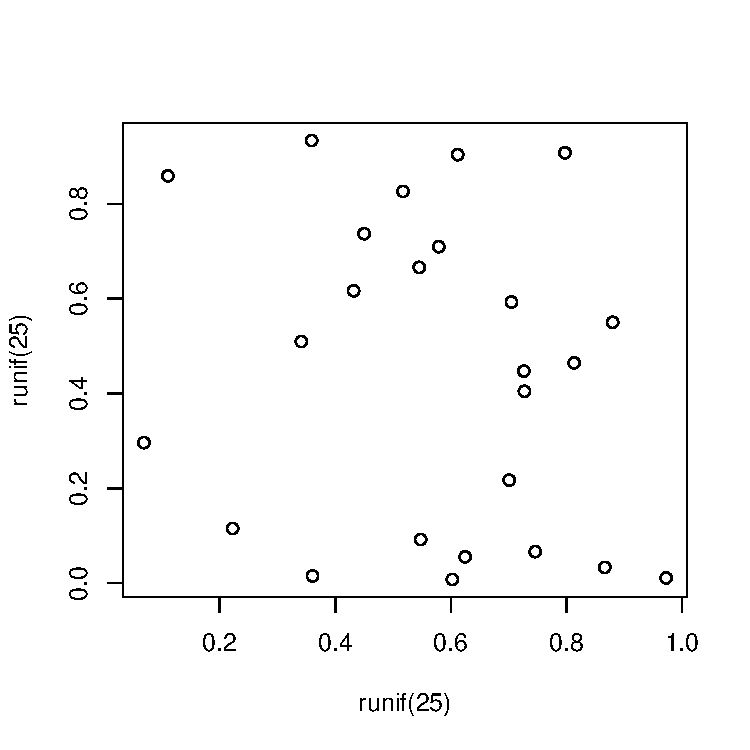
\includegraphics[width=0.5\linewidth]{testrticles_files/figure-latex/fig2-1} 

}

\caption{\label{fig2}A meaningless scatterplot.}\label{fig:fig2}
\end{figure}

\section{Tables coming from R}\label{tables-coming-from-r}

Tables can also be generated using R chunks, as shown in Table
\ref{tab1} for example.

\begin{Shaded}
\begin{Highlighting}[]
\NormalTok{knitr}\SpecialCharTok{::}\FunctionTok{kable}\NormalTok{(}\FunctionTok{head}\NormalTok{(mtcars)[,}\DecValTok{1}\SpecialCharTok{:}\DecValTok{4}\NormalTok{], }
    \AttributeTok{caption =} \StringTok{"}\SpecialCharTok{\textbackslash{}\textbackslash{}}\StringTok{label\{tab1\}Caption centered above table"}
\NormalTok{)}
\end{Highlighting}
\end{Shaded}

\begin{longtable}[]{@{}lrrrr@{}}
\caption{\label{tab1}Caption centered above table}\tabularnewline
\toprule\noalign{}
& mpg & cyl & disp & hp \\
\midrule\noalign{}
\endfirsthead
\toprule\noalign{}
& mpg & cyl & disp & hp \\
\midrule\noalign{}
\endhead
\bottomrule\noalign{}
\endlastfoot
Mazda RX4 & 21.0 & 6 & 160 & 110 \\
Mazda RX4 Wag & 21.0 & 6 & 160 & 110 \\
Datsun 710 & 22.8 & 4 & 108 & 93 \\
Hornet 4 Drive & 21.4 & 6 & 258 & 110 \\
Hornet Sportabout & 18.7 & 8 & 360 & 175 \\
Valiant & 18.1 & 6 & 225 & 105 \\
\end{longtable}

\renewcommand\refname{References}
\bibliography{mybibfile.bib}


\end{document}
